\documentclass[11pt]{article}

% Use the following to compile
% mkdir tmp
% pdflatex -aux-directory=tmp -output-directory=tmp --shell-escape notes.tex

% Package use definitions
\usepackage[margin=1in]{geometry} \usepackage{fancyhdr}
\usepackage[parfill]{parskip} \usepackage{graphicx} \usepackage{comment}
\usepackage[outputdir=tmp]{minted} \usepackage[dvipsnames]{xcolor}
\usepackage{listings} \usepackage[hidelinks]{hyperref} \usepackage{amsmath}
\usepackage{amsfonts} \usepackage{amssymb} \usepackage{tcolorbox}
\usepackage{tabu} \usepackage{upgreek} \usepackage[ruled,vlined]{algorithm2e}
\usepackage[nottoc]{tocbibind} \usepackage{natbib}

\setlength{\parindent}{11pt} \setlength{\parskip}{0pt}

% Header and footer setup
\pagestyle{fancy} \rhead{\today} \lhead{ALGOREP Project}
\renewcommand{\headrulewidth}{1pt} \renewcommand{\footrulewidth}{1pt}

% Image directory specification
\graphicspath{ {./images/} }

% Settings minted option for the entire document
\setminted{frame=lines,framesep=2mm,linenos,
  fontsize=\footnotesize
}

% Start of document
\begin{document}

% Title page and table of contents setup
\begin{titlepage}
  \begin{center}
    \vspace*{1cm} \Huge \textbf{ALGOREP Project}\\
    \vspace*{2\baselineskip} \large \textbf{Abstract}
    \vspace*{2\baselineskip}
  \end{center}
  \begin{center}
    \vfill\normalsize \textbf{Gwenegan Bertho}\\ \normalsize \textbf{Kévin
      Guillet}\\ \normalsize \textbf{Mathieu Tammaro}\\ \normalsize \textbf{Jose
      A. Henriquez Roa}\\
    \vspace*{2\baselineskip} \today \rhead{\today}
    \newpage
    \normalsize \tableofcontents
    \newpage
  \end{center}
\end{titlepage}
% Document Body:
\section{Software architecture}
This section shall go though all the design choses made throughout the
development of the project. First, a description of Messenger class, which fully
encapsulates the Open MPI API. Then, an overview of the MessageReceiver virtual
class, followed by a description of the 5 classes inheriting from it, and the
ReceiverManager class that takes care of managing all instanciations of the
derived classes. And finally, a brief description of the Node and Client
classes.
\subsection{Messenger}
\begin{figure}[H]
  \centering
  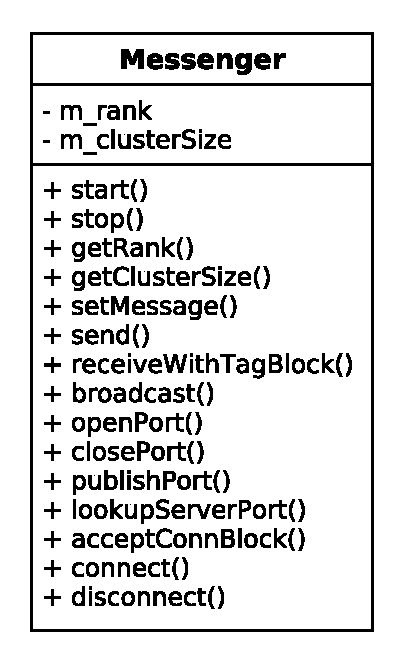
\includegraphics[scale=0.5]{image/messenger.pdf}
  \caption{Messenger class diagram}
\end{figure}
The messenger class, located in \texttt{src/include/messenger.hh}, is a complete
encapsulation of the Open MPI API. All MPI related calls are through the member
functions of this class. When it comes to making use of APIs, the design choice
encapsulating them is fairly common and easily argumented. And as with any
design choice we have done this for the sake of decreasing the complexity of the
overall architecture. Thus, we list some of the benefits of this
encapsulation;\\\\First, it allowed to safely learn to use the API by
localizing any changes made to the program to a single class. Seen as no matter
how much the manual of an API is read, it remains very likely during development
that the use of a given functionality from the API that was previously used
during the early stages might no longer be desired during later stages. For
instance during the development of this project a similar scenario was
encountered were an ambiguity in the MPI standard led to an incorrect assumption
on the behavior of a function; In the 4th version of the Message-Passing
Interface Standard in section \texttt{11.9.3} detailing the client routines to
use when implementing a client/server model with MPI the standard states
that:\\\\ ``\textit{If the port exists, but does not have a pending}
MPI\_COMM\_ACCEPT \textit{, the connection attempt will eventually time out
  after an implementation-defined time, \textbf{or} succeed when the server
  calls} MPI\_COMM\_ACCEPT \textit{.In the case of a time out,}
MPI\_COMM\_CONNECT \textit{raises an error of class } MPI\_ERR\_PORT
\textit{.}''\\\\ This statement differs in the Open MPI documentation, where the
description of the function MPI\_Comm\_Connect states that:\\\\ ``\textit{The}
MPI\_Comm\_connect \textit{call must only be called after the} MPI\_Comm\_accept
\textit{call has been made by the MPI job acting as the server.}''.\\\\ As was
found during the actual use of the MPI\_Comm\_Connect the the highligted 'or' in
the quote from the standard turned out to be an exclusive 'or' where the choice
to either implement the timeout functionality or allow the 'connect' call to
complete upon 'accept' being called on the server was left to the
implementation. This meant that there would be an intrisic need to somehow
handle race conditions from the client, due to the fact that a failed 'connect'
call would eventually timout the client, which would then force the client to
exit with an MPI\_ERR\_PORT error. This was eventually resolved by making the
clients synchronize themselves though the use of an external file, located in
\texttt{etc/turn.txt}. In this scenario this incorrect assumption led to the
unforseen implementation of a client synchonization mechanism. However, if for
instance an incorect assumption had been made on the use of the MPI\_Recv,
causing the need for this call to be switched to the non-blocking variant
MPI\_Irecv. Then having encapsulated the API would then limit the modification
required to be made to a single class, instead of every line thoughout the
project where the function was used.\\\\ Another, use for encapsulating
the API is to limit the dependency to said API. For instance, if there ever came
a need to switch Open MPI to another MPI implementation then there would only be
need to switch out the API calls on a single class instead of the entire
project. And the final use for this encapsulation is to simply hide as much
logic related to the API as possible from outside classes. And so be able to
work on other sections of the project without having to keep in mind the usage
of the API and its functionalities. And so, reduce the overall complexity of the
design.
\subsection{Receiver}
The following sections are all of the classes related to the
\texttt{MessageReceiver} class, including this one.
\subsubsection{MessageReceiver}
\begin{figure}[H]
  \centering
  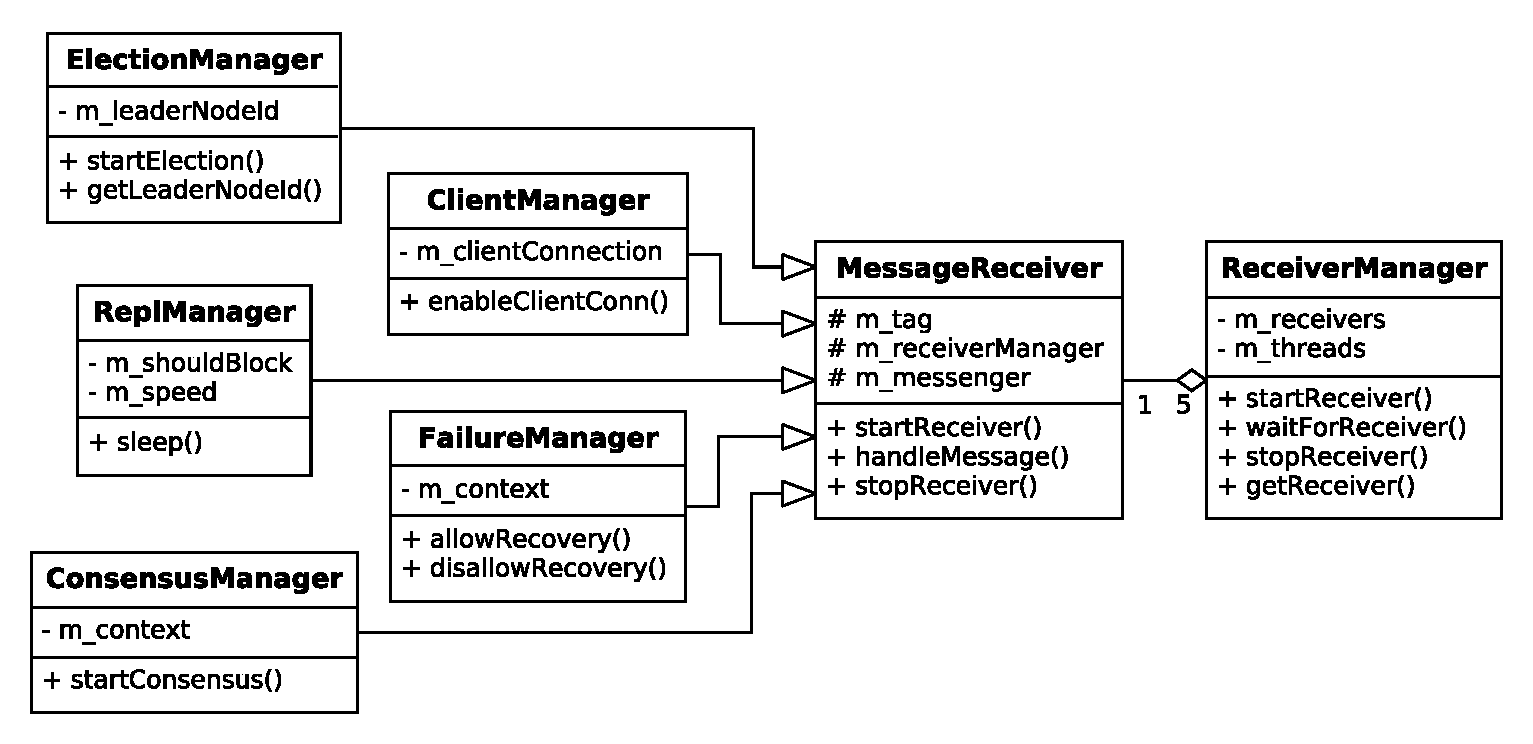
\includegraphics[scale=0.5]{image/receiver.pdf}
  \caption{MessageReceiver class diagram}
\end{figure}
The MessageReceiver class is the virtual class at the center of the class
architecture of the whole project. This class encapsulates all logic related to
receiving and handling all messages from a single specified tag. This tag is
specified in the constructor and is stored in the protected \texttt{m\_tag}
member variable. For the most part derived instances of this class, first
specify the tag to handle, and simply start an infinit 'receive' loop when the
\texttt{startReceiver()} function is called. In this loop the virtual
\texttt{handleMessage()} member function is called after each new message. And
so, derived classes only need to implement said \texttt{handleMessage()}
function.\\\\ In this project there are five different message tags. And
each of these tags possesses it's own respective set of \textit{message
  codes}. All of which are defined in the \texttt{src/include/message-info.hh}
header file. As mentioned, each of these tags are managed by their respective
\textit{Manager} inheriting from \texttt{MessageReceiver} class. The relations
are as follows:\\
\begin{minted}{c++}
  enum class MessageTag {
    LEADER_ELECTION = 0,   // ElectionManager
    CONSENSUS = 1,         // ConsensusManager
    REPL = 2,              // ReplManager
    FAILURE_DETECTION = 3, // FailureManager
    CLIENT = 4,            // ClientManager
    SIZE = 5
  };
\end{minted}
\ \\
Each of these five tag managers/receivers are instanciated once at the start of
the program and are subscribed to the \texttt{ReceiverManager}. A description of
this class and the five tag managers is given in the following sections.
\subsubsection{ReceiverManager}
As will be further detailed in the five subsequent sections each of the tag
managers has some form of time sensitive logic to handle. In most of these
sections there is need to wait for a given amount time. However, pausing the
main thread for that given amount of time could possible entail an incorect
behaviour on some other time senstive section. And so for each of these time
sensitive sections we were faced with one of two choices. Either manually
implementing said time sensitive logic through the use of busy waiting functions
or making use of multithreading and pause current the thread to let the job
scheduler switch out to an active thread. The choice was made to make use of
multithreading due to the number of time sensitive sections that were to be
implemeted which when coupled with the implementation of a specfic busy waiting
function for each of these sections would lead to a much greater amount of code
to both write and maintain.\\\\ The \texttt{ReceiverManager} class is the one
that manages these threads. One is created for each receiver and remains active
until the program is issued to shutdown, handles to these threads are stored in
the \texttt{m\_threads} member variable. In addition to this the
\texttt{ReceiverManager} also server as a container of each of the five
receivers. Access from whithing each of the receivers to other ones is done
through the use of the \texttt{getReceiver()} member function of this class.
\subsubsection{ConsensusManager}
The ConsensusManager is a derived class from the MessageReceiver handling all
messages tagged with \texttt{MessageTag::CONSENSUS}. This class only exposes a
single \texttt{startConsensus()} function. The implementation of this class is
located in \texttt{src/manager/consensus-manager.cc}. As with all classes an
effort was made to hide as much of the inner logic as possible and reduce
coupling of this class to other ones.\\
\begin{itemize}
\item \texttt{startConsensus()}: This function starts an consensus round. For the
consensus our implementation of the Multi-Paxos algorithm was used. This
function implements the behaviour of a Proposer in the Paxos algorithm. In other
words, depending on whether the respective conditions are met, it broadcasts
\texttt{PREPARE}, \texttt{PROMISE} and \texttt{ACCEPTED} (from the
\texttt{ConsensusCode} enum) to the acceptors.  While also waiting for the
respective responses for the respective given amounts of time.\\
\item \texttt{handleMessage()}: The ConsensusManager's implementation of this
  function handles the Acceptor (and Learner) side of the Paxos
  algorithm. Meaning that upon receiving the respective messages and checking
  that some additional conditions are met, it sends \texttt{PROMISE} and
  \texttt{ACCEPT} back to the proposer.\\
\end{itemize}
That said, our implementation of this algorithm is a straightforward one.
\subsubsection{ElectionManager}
The ElectionManager is the derived class from the MessageReceiver and handles
all messages tagged with \texttt{MessageTag::LEADER\_ELECTION}. When first
starting the receive loop this manager will startup an election to set the
initial leader. This class exposes the two \texttt{startElection()} and
\texttt{getLeaderNodeId()} member functions.\\
\begin{itemize}
\item \texttt{startElection()}: As the name implies this
function starts an election. For leader election the Bully algorithm was
used. This function broadcast a \texttt{ELECTION} message to all other nodes and
then waits for a victory message. If none is received for the alloted amount of
time (and no response was heard back from a node with a higher id), then a
\texttt{VICTORY} message will be broadcasted.\\
\item \texttt{handleMessage()}: Upon receival of the two election codes list above
the this function will either send back an \texttt{ALIVE} message, and possibly
start an election (depending on the id of the source node). Or simply set the
inner \texttt{m\_leaderNodeId} member variable.\\
\item \texttt{getLeaderNodeId()}: This function simply return the leader node
id. This function is only used in the FailureManager for determining whether the
current node should handle the recovery of a failed node.
\end{itemize}
\subsubsection{FailureManager}
The FailureManager is the derived class from the MessageReceiver that handles
all messages tagged with \texttt{MessageTag::FAILURE\_DETECTION}. In this case
most of the logic run by this class is done without outer interaction from other
classes in a \texttt{pingCheck()} thread created when the receive loop is first
started. Aside from this one the class exposes the two \texttt{allowRecovery()}
and \texttt{disallowRecovery()}.\\
\begin{itemize}
  \item \texttt{handleMessage()}: For the FailureManager this function handles
    four different codes presented in the following list, the last three being
    related to node recovery:\\
    \begin{enumerate}
    \item \texttt{PING}: When a ping is received. Then the respective value in a
      'last-seen' list of time points is updated for the source node. This list
      is then checked in the \texttt{pingCheck} thread.\\
      \item \texttt{STATE}: This failure code is used when sending the current
        state of the system to a recovering node. When received the node simply
        overwrites the log data with the presented one inside the message. Only
        the current leader is allowed to send this code.\\
      \item \texttt{STATE\_UDPATED}: This is the answer the recovering node
        sends back to the source node after having finished copying the new log
        state.\\
      \item \texttt{RECOVRED}: And finally, this is the message code broadcasted
        to all nodes when the node having issued the \texttt{STATE} code
        receives a \texttt{STATE\_UDPATED} from the recovering node. This and
        the two previous message codes are coupled with a 'recovery id' to
        ensure correct behavior even during a change of leader.\\
    \end{enumerate}
\item \texttt{pingCheck()}: Failure detection is done through all-to-all
  heartbeating. This function is run on a separate thread it executes an infinit
  loop that both broadcasts pings and check the 'last-seen' list at regular
  intervals. When either a failure or recovery is detected an additional
  (detached) thread is spawned to handle either event. This is done in order to
  minimize any latency these events could generate on the \texttt{pingCheck}
  thread.\\
\item \texttt{allowRecovery()}: This functions is called by the clientManager to
  notify to the failureManager that there is no current active client connection
  (which by extension means that the log will not change from this point
  on). And that any pending recovery can start from this point on.\\
\item \texttt{disallowRecovery()}: Also called by the clientManager it will
  notify the failureManager about the opposite. It will also block until the
  current recovery is done or the alloted time runs out.
\end{itemize}
\subsubsection{ClientManager}
The ClientManager is the derived class from the MessageReceiver that handles all
messages tagged with \texttt{MessageTag::CLIENT}. This class only exposes the
\texttt{enableClientConn()} member function.\\
\begin{itemize}
  \item \texttt{handleMessage()}: For the ClietnManager this function handles
    two codes \texttt{REPLICATE} and \texttt{DISCONNECT}. These respectively
    start a consensus round or notify the manager to disconnect the client. Once
    the consensus round has finished the manager responds back with
    \texttt{SUCCESS} to the client.\\
  \item \texttt{enableClientConn()}: Only the leader is allowed to allowed to
    accept client connection this is due to the nature of Multi-Paxos. This
    function is called by the ElectionManager when the current node is chosen as
    the leader.\\
\end{itemize}
\subsubsection{ReplManager}
The ReplManager is the derived class from the MessageReceiver that handles all
messages tagged with \texttt{MessageTag::REPL}. This manager is somewhat
different than the others. A greater deal of effort was made minimize the
coupling from this class to the rest of the project. This meanly been due to the
fact that on it's own it implements a completely separate set of functionalities
that are unrelated to all others. And so, the class architecture design was made
to make the removal of this particular class as easy as possible if there ever
came a need.\\ With this in mind, during development of this class we faced the
choice to; either separate an repl process from the node cluster and implement
an repl client that would read from standard input and forward the messages to
the repl process on the server, or, make the repl manager read from commands
from a file instead and keep the node cluster intact. Due to the aforementioned
reason the later option was chosen. Finally, the class itself exposes a single
\texttt{sleep()} member function.\\
\begin{itemize}
\item \texttt{handleMessage()}: This function handles the repl codes
  \texttt{START}, \texttt{SPEED\_<LOW/MEDIUM/HIGH>}, \texttt{CRASH} and
  \texttt{RECOVER}.\\
\item \texttt{sleep()}: Depending on the issued repl commands this function will
  either block the currect thread, until \texttt{RECOVERY} is received. Or put
  the thread to sleep for a given amount of time depending on whether
  \texttt{SPEED\_<LOW/MEDIUM/HIGH>} were received. This function is called by
  all receivers except this one right before their respective
  \texttt{handleMessage()} function.
\end{itemize}
\section{Tests}
Testing was exclusively done by hand through the use of debug messages rather
than through a streamlined test suit. This is due to the multithreaded nature of
the application and to our belief that setting up such a system would require a
too large of a portion of the emparted time. The following presents some of the
debug messages that were used during development:\\\\
\texttt{[0][0][1]: \{"code":1\}}\\
\texttt{[0][0][2]: \{"code":1\}}\\
\texttt{[0][1][2]: \{"code":1\}}\\
\texttt{[0][2][0]: \{"code":2\}}\\
\texttt{[0][1][0]: \{"code":2\}}\\
\texttt{[0][1][2]: \{"code":1\}}\\
\texttt{[0][2][1]: \{"code":2\}}\\
\texttt{[0][2][1]: \{"code":2\}}\\
\texttt{[0][2][0]: \{"code":3\}}\\
\texttt{[0][2][1]: \{"code":3\}}\\\\
It shows an election between three nodes. The number between the first first set
of brackets show the tag \texttt{MessageTag::LEADER\_ELECTION} in this case and
the following two sets of brackets respectively show the source node id and the
destination node id of the message. What follows is the message code in json
format. The mapping between the integer and what it means is as follows:
\begin{minted}{c++}
  enum class LeaderElectionCode {
    SHUTDOWN = 0,
    ELECTION = 1,
    ALIVE = 2,
    VICTORY = 3
  };
\end{minted}
\section{Performance measures}
\end{document}
